%%%%%%%%%%%%%%%%%%%%%%%%%%%%%%%%%%%%%%%%%%%%%%%%%%%%%%%%%%%%%%%%%%%%%%%%%%%%%%%
%Tutorial slides on Python.
%
% Author: FOSSEE
% Copyright (c) 2009, FOSSEE, IIT Bombay
%%%%%%%%%%%%%%%%%%%%%%%%%%%%%%%%%%%%%%%%%%%%%%%%%%%%%%%%%%%%%%%%%%%%%%%%%%%%%%%%

\documentclass[14pt,compress]{beamer}
%\documentclass[draft]{beamer}
%\documentclass[compress,handout]{beamer}
%\usepackage{pgfpages} 
%\pgfpagesuselayout{2 on 1}[a4paper,border shrink=5mm]

% Modified from: generic-ornate-15min-45min.de.tex
\mode<presentation>
{
  \usetheme{Warsaw}
  \useoutertheme{infolines}
  \setbeamercovered{transparent}
}

\usepackage[english]{babel}
\usepackage[latin1]{inputenc}
%\usepackage{times}
\usepackage[T1]{fontenc}

% Taken from Fernando's slides.
\usepackage{ae,aecompl}
\usepackage{mathpazo,courier,euler}
\usepackage[scaled=.95]{helvet}

\definecolor{darkgreen}{rgb}{0,0.5,0}

\usepackage{listings}
\lstset{language=Python,
    basicstyle=\ttfamily\bfseries,
    commentstyle=\color{red}\itshape,
  stringstyle=\color{darkgreen},
  showstringspaces=false,
  keywordstyle=\color{blue}\bfseries}

%%%%%%%%%%%%%%%%%%%%%%%%%%%%%%%%%%%%%%%%%%%%%%%%%%%%%%%%%%%%%%%%%%%%%%
% Macros
\setbeamercolor{emphbar}{bg=blue!20, fg=black}
\newcommand{\emphbar}[1]
{\begin{beamercolorbox}[rounded=true]{emphbar} 
      {#1}
 \end{beamercolorbox}
}
\newcounter{time}
\setcounter{time}{0}
\newcommand{\inctime}[1]{\addtocounter{time}{#1}{\tiny \thetime\ m}}

\newcommand{\typ}[1]{\lstinline{#1}}

\newcommand{\kwrd}[1]{ \texttt{\textbf{\color{blue}{#1}}}  }

\newcommand{\num}{\texttt{numpy}}

%%% This is from Fernando's setup.
% \usepackage{color}
% \definecolor{orange}{cmyk}{0,0.4,0.8,0.2}
% % Use and configure listings package for nicely formatted code
% \usepackage{listings}
% \lstset{
%    language=Python,
%    basicstyle=\small\ttfamily,
%    commentstyle=\ttfamily\color{blue},
%    stringstyle=\ttfamily\color{orange},
%    showstringspaces=false,
%    breaklines=true,
%    postbreak = \space\dots
% }


%%%%%%%%%%%%%%%%%%%%%%%%%%%%%%%%%%%%%%%%%%%%%%%%%%%%%%%%%%%%%%%%%%%%%%
% Title page
\title[Interactive Plotting]{Introductory Scientific Computing with
Python}
\subtitle{More plotting, lists and numpy arrays}

\author[Prabhu] {FOSSEE}

\institute[FOSSEE -- IITB] {Department of Aerospace Engineering\\IIT Bombay}
\date[] {PyCon Asia-Pacific,\\
Singapore\\
June 9, 2011
}

%%%%%%%%%%%%%%%%%%%%%%%%%%%%%%%%%%%%%%%%%%%%%%%%%%%%%%%%%%%%%%%%%%%%%%

%\pgfdeclareimage[height=0.75cm]{iitmlogo}{iitmlogo}
%\logo{\pgfuseimage{iitmlogo}}


%% Delete this, if you do not want the table of contents to pop up at
%% the beginning of each subsection:
\AtBeginSubsection[]
{
  \begin{frame}<beamer>
    \frametitle{Outline}
    \tableofcontents[currentsection,currentsubsection]
  \end{frame}
}

\AtBeginSection[]
{
  \begin{frame}<beamer>
    \frametitle{Outline}
    \tableofcontents[currentsection,currentsubsection]
  \end{frame}
}

% If you wish to uncover everything in a step-wise fashion, uncomment
% the following command: 
%\beamerdefaultoverlayspecification{<+->}

%\includeonlyframes{current,current1,current2,current3,current4,current5,current6}

%%%%%%%%%%%%%%%%%%%%%%%%%%%%%%%%%%%%%%%%%%%%%%%%%%%%%%%%%%%%%%%%%%%%%%
% DOCUMENT STARTS
\begin{document}

\begin{frame}
  \titlepage
\end{frame}

\begin{frame}
  \frametitle{Outline}
  \tableofcontents
  % You might wish to add the option [pausesections]
\end{frame}

\section{Plotting Points}
\begin{frame}[fragile]
\frametitle{Why would I plot f(x)?}
Do we plot analytical functions or experimental data?
\begin{small}
\begin{lstlisting}
In []: time = [0, 1, 2, 3]

In []: distance = [7, 11, 15, 19]

In []: plot(time,distance)
Out[]: [<matplotlib.lines.Line2D object at 0xa73aa8c>]

In []: xlabel('time')
Out[]: <matplotlib.text.Text object at 0x986e9ac>

In []: ylabel('distance')
Out[]: <matplotlib.text.Text object at 0x98746ec>
\end{lstlisting}
\end{small}
\end{frame}

\begin{frame}[fragile]
\begin{figure}
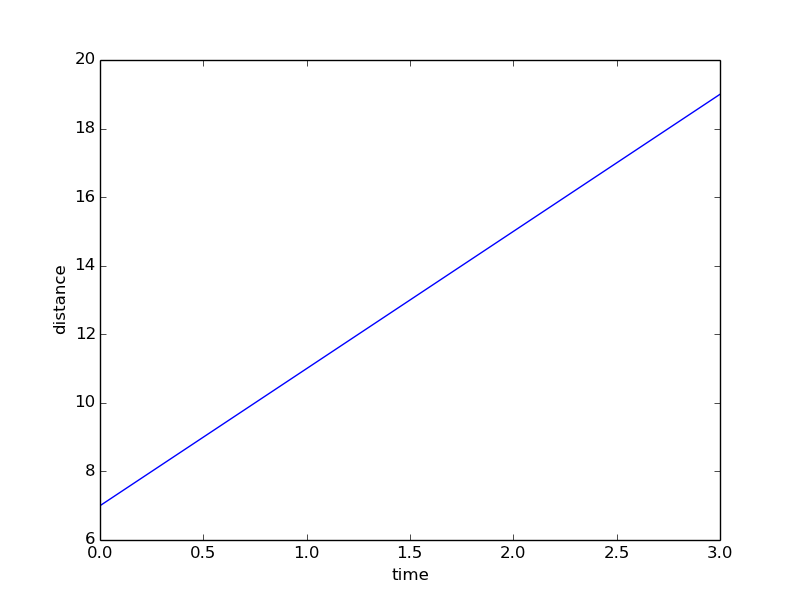
\includegraphics[width=3.5in]{data/straightline.png}
\end{figure}
\alert{Is this what you have?}
\end{frame}

\begin{frame}[fragile]
\frametitle{Plotting points}
\begin{itemize}
\item What if we want to plot the points?
\end{itemize}
\begin{lstlisting}
  In []: clf()

  In []: plot(time, distance, 'o')
  Out[]: [<matplotlib.lines.Line2D object at 0xac17e0c>]

  In []: clf()
  In []: plot(time, distance, '.')
  Out[]: [<matplotlib.lines.Line2D object at 0xac17e0c>]
\end{lstlisting}
\end{frame}

\begin{frame}[fragile]
\begin{figure}
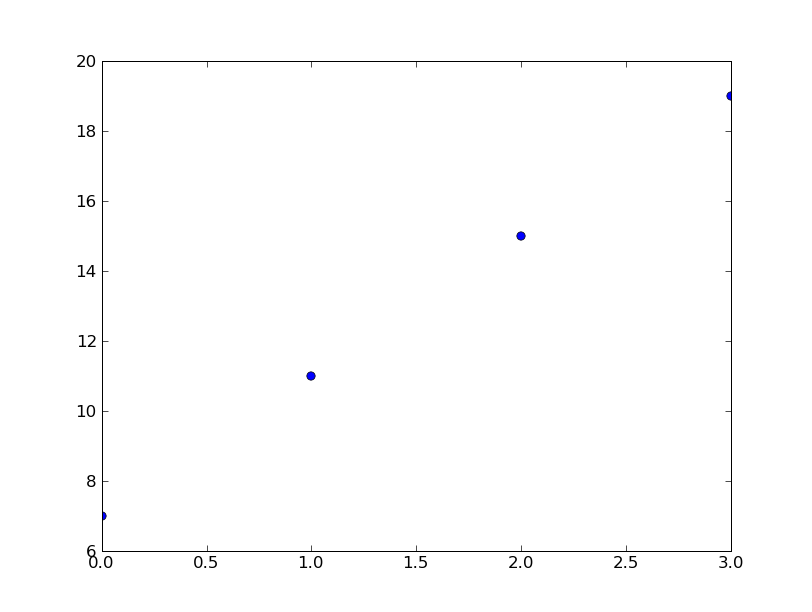
\includegraphics[interpolate=true,width=2.35in]{data/stline_dots.png}
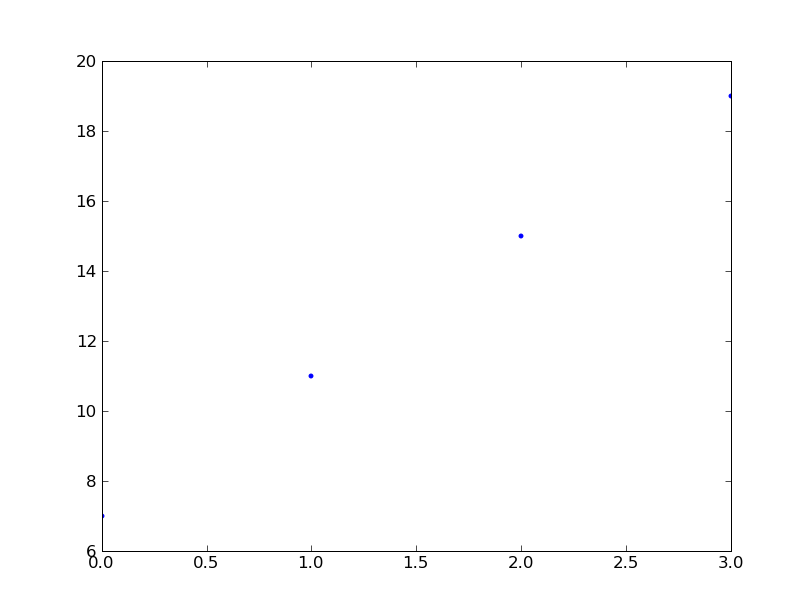
\includegraphics[interpolate=true,width=2.35in]{data/stline_points.png}
\end{figure}
\end{frame}

\begin{frame}[fragile]
\frametitle{Additional Line Styles}
\begin{itemize}
  \item \typ{'o'} - Filled circles
  \item \typ{'.'} - Small Dots
  \item \typ{'-'} - Lines
  \item \typ{'--'} - Dashed lines
\end{itemize}
\end{frame}

\section{Lists}
\begin{frame}[fragile]
  \frametitle{Lists: Introduction}
  \begin{lstlisting}
    In []: time = [0, 1, 2, 3]

    In []: distance = [7, 11, 15, 19]

  \end{lstlisting}
What are \typ{x} and \typ{y}?\\
\begin{center}
\alert{\typ{lists!!}}
\end{center}
\end{frame}

\begin{frame}[fragile]
\frametitle{Lists: Initializing \& accessing elements}
\begin{lstlisting}
In []: mtlist = [] 
\end{lstlisting}
\emphbar{Empty List}
\begin{lstlisting}
In []: p = [ 2, 3, 5, 7] 

In []: p[1]
Out[]: 3

In []: p[0]+p[1]+p[-1]
Out[]: 12
\end{lstlisting}
\end{frame}

\begin{frame}[fragile]
  \frametitle{List: Slicing}
  \begin{block}{Remember\ldots}
	\kwrd{In []: p = [ 2, 3, 5, 7]}
  \end{block}
\begin{lstlisting}
In []: p[1:3]
Out[]: [3, 5]
\end{lstlisting}
\emphbar{A slice}
\begin{lstlisting}
In []: p[0:-1]
Out[]: [2, 3, 5]
In []: p[1:]
Out[]: [3, 5, 7]
\end{lstlisting}
\end{frame}

\begin{frame}[fragile]
  \frametitle{List: Slicing \ldots}
\begin{lstlisting}
In []: p[0:4:2]
Out[]: [2, 5]
In []: p[0::2]
Out[]: [2, 5]
In []: p[::2]
Out[]: [2, 5]
In []: p[::3]
Out[]: [2, 7]
In []: p[::-1]
Out[]: [7, 5, 3, 2]
\end{lstlisting}
\alert{\typ{list[initial:final:step]}}
\end{frame}

\begin{frame}[fragile]
  \frametitle{List: Slicing}
  What is the output of the following?
\begin{lstlisting}
In []: p[1::2]

In []: p[1:-1:2]
\end{lstlisting}
\end{frame}


%% more on list slicing
\begin{frame}[fragile]
\frametitle{List operations}
\begin{lstlisting}
In []: b = [ 11, 13, 17]
In []: c = p + b

In []: c
Out[]: [2, 3, 5, 7, 11, 13, 17]

In []: p.append(11)
In []: p
Out[]: [ 2, 3, 5, 7, 11]
\end{lstlisting}
Question: Does \typ{c} change now that \typ{p} is changed?
\inctime{10}
\end{frame}

\section{Simple Pendulum}
\begin{frame}[fragile]
\frametitle{Simple Pendulum - L and T}
Let us look at the Simple Pendulum experiment.
\begin{center}
\begin{small}
\begin{tabular}{| c | c | c |}
\hline
$L$ & $T$ & $T^2$ \\ \hline
0.1 & 0.69 & \\ \hline
0.2 & 0.90 & \\ \hline
0.3 & 1.19 & \\ \hline
0.4 & 1.30 & \\ \hline
0.5 & 1.47 & \\ \hline
0.6 & 1.58 & \\ \hline
0.7 & 1.77 & \\ \hline
0.8 & 1.83 & \\ \hline
0.9 & 1.94 & \\ \hline
\end{tabular}
\end{small}\\
\alert{$L \alpha T^2$}
\end{center}
\end{frame}

\begin{frame}[fragile]
\frametitle{Lets use lists}
\begin{lstlisting}
In []: L = [0.1, 0.2, 0.3, 0.4, 0.5, 
            0.6, 0.7, 0.8, 0.9]

In []: t = [0.69, 0.90, 1.19, 
            1.30, 1.47, 1.58, 
            1.77, 1.83, 1.94]
\end{lstlisting}
\alert{Gotcha}: Make sure \typ{L} and \typ{t} have the same number
of elements

\begin{lstlisting}
In []: print len(L), len(t)
\end{lstlisting}

\end{frame}

\begin{frame}[fragile]
\frametitle{Plotting $L$ vs $T^2$}
\begin{itemize}
\item We must square each of the values in \typ{t}
\item How do we do it?
\item We use a \kwrd{for} loop to iterate over \typ{t}
\end{itemize}
\end{frame}

\begin{frame}[fragile]
\frametitle{Plotting $L$ vs $T^2$}
\begin{lstlisting}
In []: tsq = []

In []: for time in t:
 ....:     tsq.append(time*time)
 ....:
 ....:

\end{lstlisting}
This gives \typ{tsq} which is the list of squares of \typ{t} values.
\begin{lstlisting}
In []: print len(L), len(t), len(tsq)
Out[]: 9 9 9

In []: plot(L, tsq)
\end{lstlisting}
\end{frame}

\begin{frame}[fragile]
\begin{figure}
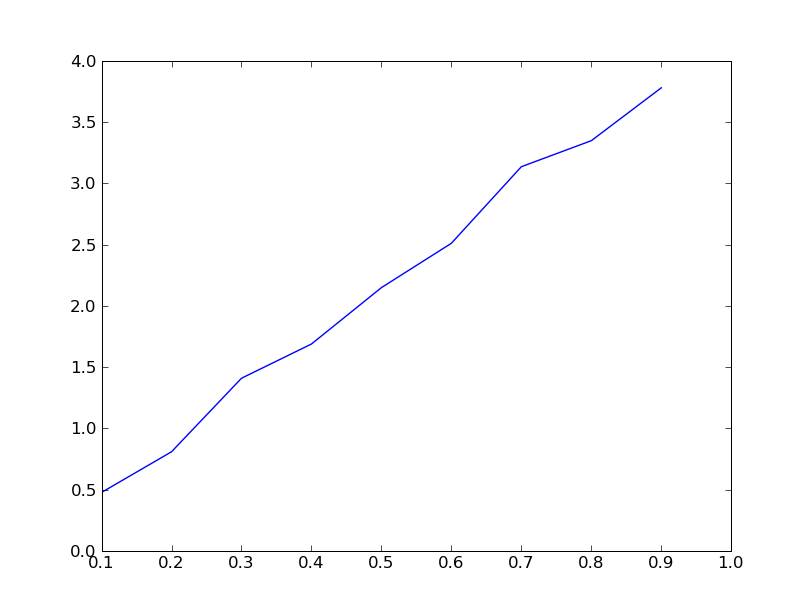
\includegraphics[width=3.5in]{data/L-TSq-limited.png}
\end{figure}
\end{frame}


\begin{frame}[fragile]
\frametitle{This seems tedious}
\begin{itemize}
    \item Lists
\begin{itemize}
    \item Nice
    \item Not too convenient 
    \item Slow
\end{itemize}
\item Enter NumPy arrays
    \begin{itemize}
        \item Fixed size, data type
        \item Fast
        \item Very convenient
    \end{itemize}
\end{itemize}
\end{frame}

\subsection{\num\ arrays}

\begin{frame}[fragile]
\frametitle{NumPy arrays}
\begin{lstlisting} 
In []: t = array(t)

In []: tsq = t*t

In []: print tsq

In []: plot(L, tsq) # works!
\end{lstlisting}  %$
\end{frame}


\begin{frame}[fragile]
\frametitle{Speed?}

\noindent Lets use range to create a large list.

\begin{lstlisting} 
In []: t = range(1000000)
In []: tsq = []

In []: for time in t:
 ....:     tsq.append(time*time)
 ....:
 ....:
\end{lstlisting}  %$

\noindent Now try it with 

\begin{lstlisting}
In []: t = array(t)

In []: tsq = t*t
\end{lstlisting}
\ldots
\end{frame}

\begin{frame}[fragile]
\frametitle{How fast is this?}
\noindent Lets define a function for the list
\begin{lstlisting}
In []: def sqr(arr):
  ...:     ret = []
  ...:     for x in arr:
  ...:         ret.append(x*x)
  ...:     return ret
  ...: 

In []: tsq = sqr(t)

\end{lstlisting}  %$
\end{frame}

\begin{frame}[fragile]
  \frametitle{IPython tip: Timing}

Try the following:
  \begin{lstlisting}
In []: %timeit sqr(t) 

In []: %timeit?

  \end{lstlisting}

  \begin{itemize}
      \item \typ{\%timeit}: accurate, many measurements
      \item Can also use \typ{\%time}
      \item \typ{\%time}: less accurate, one measurement 
  \end{itemize}

\inctime{15}
\end{frame}


\begin{frame}[fragile]
\frametitle{Exercise}
\begin{center}
    Find out the speed difference between the \typ{sqr} function and
    \typ{t*t} on the numpy array.
\end{center}

\end{frame}

\begin{frame}[fragile]
  \frametitle{The \num\ module}
    \begin{itemize}
    \item Efficient, powerful array type
    \item Abstracts out standard operations on arrays
    \item Convenience functions
    \item \typ{ipython --pylab} imports part of numpy
    \item Without the Pylab mode do:
    \end{itemize}
    \begin{lstlisting}
In []: import numpy

In []: from numpy import *
    \end{lstlisting}
\end{frame}

\begin{frame}
  \frametitle{\num\ arrays}
  \begin{itemize}
  \item Fixed size (\typ{arr.size})
  \item Same type (\typ{arr.dtype})
  \item Arbitrary dimensionality: \typ{arr.shape}
  \item \typ{shape}: extent (size) along each dimension
  \item \typ{arr.itemsize}: number of bytes per element
  \item \alert{Note:} \typ{shape} can change so long as the \typ{size}
      is constant
  \item Indices start from 0
  \item Negative indices do the right thing.
  \end{itemize}
\end{frame}

\begin{frame}[fragile]
  \frametitle{\num\ arrays}
\begin{lstlisting}
In []: a = array([1,2,3,4])
In []: b = array([2,3,4,5])

In []: print a[0], a[-1]
1, 4

In []: a[0] = -1
In []: a[0] = 1
\end{lstlisting}
Operations are elementwise
\end{frame}

\begin{frame}[fragile]
  \frametitle{Simple operations}
\begin{lstlisting}
In []: a + b  
Out[]: array([3, 5, 7, 9])
In []: a*b
Out[]: array([2, 6, 12, 20])
In []: a/b
Out[]: array([0, 0, 0, 0])
\end{lstlisting}
Operations are elementwise, types matter.
\end{frame}

\begin{frame}[fragile]
  \frametitle{Data type matters}
  Try again with this:
\begin{lstlisting}
In []: a = array([1.,2,3,4])
In []: a/b 
\end{lstlisting}
\end{frame}

\begin{frame}[fragile]
  \frametitle{Examples}
\noindent \typ{pi} and \typ{e} are defined.
\begin{lstlisting}
In []: x = linspace(0.0, 10.0, 200)
In []: x *= 2*pi/10
# apply functions to array.
In []: y = sin(x)
In []: y = cos(x)
In []: x[0] = -1
In []: print x[0], x[-1]
-1.0 10.0
\end{lstlisting}
\end{frame}

\begin{frame}[fragile]
    \frametitle{\typ{size, shape, rank} etc.}
\vspace*{-8pt}
\begin{lstlisting}
In []: x = array([1., 2, 3, 4])
In []: size(x)
Out[]: 4
In []: x.dtype
dtype('float64')
In []: x.shape
Out[] (4,)
In []: rank(x)
Out[]: 1
In []: x.itemsize
Out[]: 8
\end{lstlisting}
\end{frame}


\begin{frame}[fragile]
  \frametitle{Multi-dimensional arrays}
\begin{lstlisting}
In []: a = array([[ 0, 1, 2, 3],
  ...:            [10,11,12,13]])
In []: a.shape # (rows, columns)
Out[]: (2, 4)

In []: a[1,3] 
Out[]: 13

In []: a[1,3] = -1
In []: a[1] # The second row
array([10,11,12,-1])
In []: a[1] = 0 # Entire row to zero.
\end{lstlisting}

\end{frame}

\begin{frame}[fragile]
  \frametitle{Slicing arrays}
  \vspace*{-0.2in}
\begin{lstlisting}
In []: a = array([[1,2,3], [4,5,6], 
  ...:            [7,8,9]])
In []: a[0,1:3]
Out[]: array([2, 3])
In []: a[1:,1:]
Out[]: array([[5, 6],
              [8, 9]])
In []: a[:,2]
Out[]: array([3, 6, 9])
In []: a[0::2,0::2] # Striding...
Out[]: array([[1, 3],
              [7, 9]])
# Slices refer to the same memory!
\end{lstlisting}
\end{frame}

\begin{frame}[fragile]
  \frametitle{Array creation functions}
  \begin{itemize}
  \item \typ{array(object)}
  \item \typ{linspace(start, stop, num=50)}
  \item \typ{ones(shape)}
  \item \typ{zeros((d1,...,dn))}
  \item \typ{empty((d1,...,dn))}
  \item \typ{identity(n)}
  \item \typ{ones\_like(x)}, \typ{zeros\_like(x)}, \typ{empty\_like(x)}
  \end{itemize}
  May pass an optional \typ{dtype=} keyword argument

  For more dtypes see: \typ{numpy.typeDict}
\end{frame}

\begin{frame}[fragile]
  \frametitle{Creation examples}
  \vspace*{-0.25in}
\begin{lstlisting}
In []: a = array([1,2,3], dtype=float)
In []: ones( (2, 3) )
Out[]: array([[ 1.,  1.,  1.],
              [ 1.,  1.,  1.]])
In []: identity(3)
Out[]: array([[ 1.,  0.,  0.],
              [ 0.,  1.,  0.],
              [ 0.,  0.,  1.]])
In []: ones_like(a)
Out[]: array([ 1.,  1.,  1.,  1.])
\end{lstlisting}
\end{frame}

\begin{frame}[fragile]
  \frametitle{Array math}
  \begin{itemize}
  \item Basic \alert{elementwise} math (given two arrays \typ{a, b}):
    \begin{itemize}
        \item \typ{a + b} $\rightarrow$ \typ{add(a, b)} 
        \item \typ{a - b}, $\rightarrow$ \typ{subtract(a, b)} 
        \item \typ{a * b}, $\rightarrow$ \typ{multiply(a, b)} 
        \item \typ{a / b}, $\rightarrow$ \typ{divide(a, b)} 
        \item \typ{a \% b}, $\rightarrow$ \typ{remainder(a, b)} 
        \item \typ{a ** b}, $\rightarrow$ \typ{power(a, b)}
    \end{itemize}
  \item Inplace operators: \typ{a += b}, or \typ{add(a, b,
      a)}
    \alert{What happens if \typ{a} is \typ{int} and \typ{b} is \typ{float?}}
  \item Logical operations: \typ{==, !=, <, >}, etc.
  \item \typ{sin(x), arcsin(x), sinh(x)},
      \typ{exp(x), sqrt(x)} etc.
  \item \typ{sum(x, axis=0), product(x, axis=0)}
  \item \typ{dot(a, b)}
  \end{itemize}
\end{frame}

\begin{frame}[fragile]
    \frametitle{Convenience functions: \typ{loadtxt}}
  \begin{itemize}
      \item \typ{loadtxt(file_name)}: loads a text file 
      \item \typ{loadtxt(file_name, unpack=True)}: loads a text file and
          unpacks columns
  \end{itemize}
  \begin{lstlisting}
In []: x = loadtxt('pendulum.txt')
In []: x.shape
Out[]: (90, 2)

In []: x, y = loadtxt('pendulum.txt', 
  ...:                 unpack=True)
In []: x.shape
Out[]: (90,)
  \end{lstlisting}

  \inctime{20}
\end{frame}


\begin{frame}[fragile]
  \frametitle{Advanced}
  \begin{itemize}
  \item Only scratched the surface of \num
  \item \typ{reduce, outer}
  \item Typecasting
  \item More functions: \typ{take, choose, where}, \typ{compress,
      concatenate}
  \item Array broadcasting and \typ{None}
  \item Record arrays
  \end{itemize}
\end{frame}

\begin{frame}[fragile]
  \frametitle{Recap}
  \begin{itemize}
      \item Basic concepts: creation, access, operations
      \item 1D, multi-dimensional
      \item Slicing
      \item Array creation, dtypes
      \item Math
      \item \typ{loadtxt}
  \end{itemize}
\end{frame}

\begin{frame}[fragile]
\frametitle{Example: plotting data from file}
\alert{Data is usually present in a file!} \\
Lets look at the \typ{pendulum.txt} file.
\begin{lstlisting} 
In []: cat pendulum.txt 
1.0000e-01 6.9004e-01
1.1000e-01 6.9497e-01
1.2000e-01 7.4252e-01
1.3000e-01 7.5360e-01
\end{lstlisting}  %$
\ldots
\end{frame}

\begin{frame}[fragile]
\frametitle{Reading \typ{pendulum.txt}}
\begin{itemize}
  \item File contains L vs.\ T values 
  \item First Column - L values
  \item Second Column - T values
  \item Let us generate a plot from the data file
\end{itemize}
\end{frame}

\begin{frame}[fragile]
    \frametitle{Gotcha and an aside}
    Ensure you are in the same directory as \typ{pendulum.txt}\\
    if not, do the following on IPython:
    \begin{lstlisting}
In []: %cd directory_containing_file
# Check if pendulum.txt is there.
In []: ls
# Also try 
In []: !ls
    \end{lstlisting}

    \alert{Note:} \typ{\%cd} is an IPython magic command.  For more information
    do:
    \begin{lstlisting}
In []: ?
    \end{lstlisting}
\end{frame}


\begin{frame}[fragile]
    \frametitle{Exercise}
    \begin{itemize}
        \item Plot L versus T square with dots
        \item No line connecting points
    \end{itemize}
\end{frame}

\begin{frame}[fragile]
\frametitle{Solution}
\begin{lstlisting}
In []: L, t = loadtxt('pendulum.txt', 
 ....:                unpack=True)
In []: plot(L, t*t, '.')
\end{lstlisting}
or
\begin{lstlisting}
In []: x = loadtxt('pendulum.txt')
In []: L, t = x[:,0], x[:,1]
In []: plot(L, t*t, '.')
\end{lstlisting}

\end{frame}


\begin{frame}[fragile]
\begin{figure}
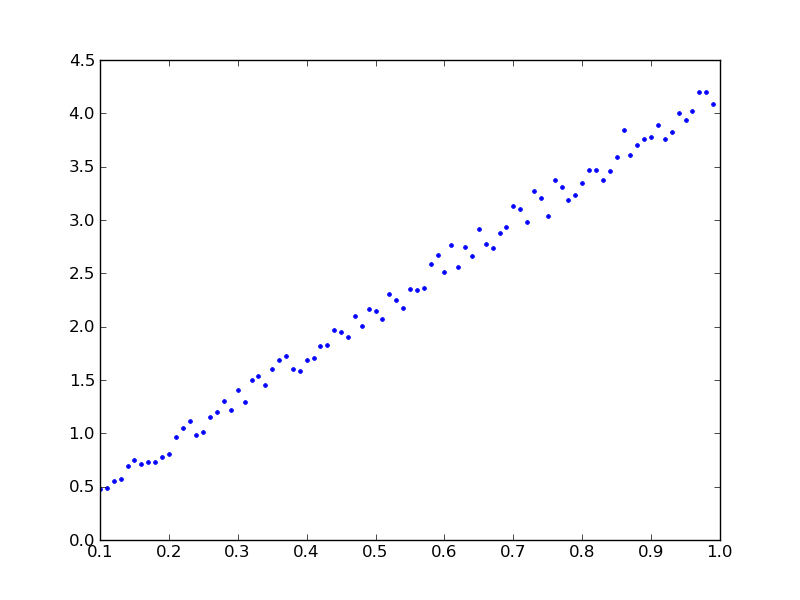
\includegraphics[width=3.5in]{data/L-Tsq.png}
\end{figure}
\end{frame}

\begin{frame}[fragile]
\frametitle{Odds and ends}
\begin{lstlisting}
In []: mean(L)
Out[]: 0.54499999999999993

In []: std(L)
Out[]: 0.25979158313283879
\end{lstlisting}
\end{frame}

\section {Summary}
\begin{frame}[fragile]
\frametitle{What did we learn?}
\begin{itemize}
  \item Plot attributes and plotting points
  \item Lists
  \item Introduction to \num\ arrays
\end{itemize}

\inctime{10}
\end{frame}

\end{document}

%% Questions for Quiz %%
%% ------------------ %%

\begin{frame}[fragile]
\frametitle{\incqno }
  \begin{lstlisting}
  In []: a = [1, 2, 5, 9]
  In []: a[0:-1]
  \end{lstlisting}
  What is the output?
\end{frame}

\begin{frame}
\frametitle{\incqno }
  How do you combine two lists \emph{a} and \emph{b} to produce one list?
\end{frame}

\begin{frame}[fragile]
\frametitle{\incqno }
  \begin{lstlisting}
  In []: a = [1, 2, 5, 9]
  \end{lstlisting}
  How do you add the value 10 to the end of this list?
\end{frame}

\begin{frame}
\frametitle{\incqno }
Write the code to read a file \texttt{data.txt} and print each line of it?
\end{frame}

\begin{frame}[fragile]
\frametitle{\incqno }
What would be the result of the following code snippet:
\begin{lstlisting}
In []: x = linspace(0, 10, 50)
In []: y = linspace(50, 100, 100)
In []: plot(x, y)
\end{lstlisting}
\end{frame}

\begin{frame}[fragile]
\frametitle{\incqno }
The following code snippet has an error/bug:
\begin{lstlisting}
In []: l = [0.1, 0.2, 0.3, 0.4]
In []: t = [0.69, 0.90, 1.19, 1.30]
In []: tsq = []
In []: for time in t:
 ....:     tsq.append(time*time)
 ....:     plot(l, tsq)
\end{lstlisting}
What is the error? How do you fix it?
\end{frame}
